\chapter{روش پیشنهادی}
%\thispagestyle{empty}

\section{مقدمه}

روش‌های موجود در زمینه یادگیری پیوسته برای داده‌های ویدیویی با وجود پیشرفت‌های اخیر، همچنان با مشکلات اساسی روبه‌رو هستند. برخی رویکردها به مدل‌های از پیش آموزش‌دیده متکی‌اند، اما برای انطباق با داده‌های ویدیویی نیاز به آموزش یا تنظیم مجدد کدگذارهای زمانی دارند، که فرآیندی زمان‌بر، پرهزینه و وابسته به منابع سخت‌افزاری سنگین است \cite{pivot}. هم‌چنین، روش‌های مختلف (تصویر یا ویدیو)، برای مقابله با فراموشی فاجعه‌بار به استفاده از بافرهای بازپخش یا ذخیره‌سازی داده‌های قبلی متکی هستند که نیازمند حافظه بالا و ناسازگار با محدودیت‌های حریم خصوصی است
\cite{pivot,9,memory-1}
. علاوه بر این، برخی از روش‌ها از ساختارهای وابسته به وظیفه
\LTRfootnote{Task specific}
استفاده می‌کنند که مدیریت و نگهداری آن‌ها در سناریوهای واقعی و وظایف متوالی دشوار بوده و باعث کاهش تعمیم‌پذیری می‌شود \cite{task-specific-1,task-specific-2}.

با توجه به این محدودیت‌ها، نیاز به رویکردهایی احساس می‌شود که بتوانند بدون وابستگی به ذخیره‌سازی وسیع داده‌های گذشته یا آموزش سنگین کدگذارها، عملکرد بهتری در داده‌های ویدیویی ارائه دهند و در عین حال ماهیت مستقل از وظیفه
\LTRfootnote{Task-agnostic}
 داشته باشند. هدف چنین رویکردهایی این است که از ظرفیت مدل‌های بزرگ و از پیش آموزش‌دیده استفاده کرده و با اضافه کردن لایه‌های سبک یا پرامپت‌های یادگیرنده، بدون تغییر مستقیم پارامتر‌های اصلی مدل، دانش قبلی را حفظ کنند و با داده‌های جدید تطبیق یابند.

در راستای رفع محدودیت‌های مذکور، در این فصل به ارائه روشی با عنوان
\lr{ProActionCLIP}\RTLfootnote{این نام مخفف \lr{Prompt Action recognition CLIP} 
	می‌باشد که به استفاده از روش‌ پرامپت‌گذاری برای تشخیص حرکت توسط مدل کلیپ، اشاره می‌کند.
}،
پرداخته‌ می‌شود که با ترکیب قابلیت‌های روش
\lr{Open-VCLIP}~\cite{open-vclip}
و ایده‌های روش
\lr{L2P}~\cite{l2p}، 
از پرامپت‌های سبک و پویا، برای انطباق با وظایف جدید، استفاده می‌کند. بنابراین در این روش، نیازی به طی کردن فرآیند آموزش کدگذارهای زمانی، که از نظر محاسباتی هزینه‌بر است، وجود ندارد.
روش \lr{ProActionCLIP}، با بهره‌گیری بهینه از دانش مدل‌های پیش‌آموزش‌دیده، کاهش فراموشی فاجعه‌بار و حفظ کارآیی در سناریوهای واقعی را هدف قرار داده است. این روش می‌تواند با بهره‌گیری بهینه از منابع محاسباتی و نیاز کمتر به سخت‌افزار، توانایی یادگیری پیوسته وظایف جدید را داشته باشد و بدون وابستگی به شناسه وظایف، عملکردی کارآمد و مقیاس‌پذیر ارائه دهد.

\section{روش \lr{ProActionCLIP}}
روش
\lr{ProActionCLIP}،
که برای یادگیری پیوسته‌ی تشخیص حرکت انسان معرفی شده، بر پایه‌ی ترکیب دو رویکرد
\lr{Open-VCLIP}
و
\lr{L2P}،
بنا شده است. ایده‌ی اصلی این روش آن است که از قابلیت‌های \lr{Open-VCLIP} برای استخراج ویژگی‌های چندماهیتی (تصویر-متن) بهره گرفته و در عین حال از سازوکار پرامپت‌های یادگیرنده در \lr{L2P} استفاده می‌کند. به‌این‌ترتیب مدل می‌تواند بدون نیاز به تغییر مستقیم پارامتر‌های کدگذار اصلی، خود را با وظایف متوالی تطبیق دهد. این ترکیب باعث می‌شود که مشکل فراموشی فاجعه‌بار کاهش یافته، حافظه‌ی مورد نیاز برای ذخیره‌سازی نمونه‌ها به حداقل برسد و مدل به صورت مستقل از وظیفه، وظایف جدید را پردازش کند. به عبارت دیگر، با این رویکرد سعی شده است مزیت‌های هر دو روش با هم ترکیب شود که عبارت‌اند از: قدرت تعمیم‌دهی و دانش وسیع \lr{Open-VCLIP} و انعطاف‌پذیری \lr{L2P} در مدیریت وظایف پیوسته. مدل \lr{ProActionCLIP}، شامل دو مرحله‌‌ی آموزش  و آزمون می‌باشد که پس از معرفی مدل‌های پایه‌‌ی بکار برده شده در
\lr{ProActionCLIP}،
به توضیح آن‌ها پرداخته می‌شود.

\section{مدل \lr{Open-VCLIP}}
مدل‌های بینایی-زبان مانند \lr{CLIP}، به دلیل توانایی یادگیری بازنمایی‌های مشترک تصویر و متن، عملکرد قابل توجهی در وظایف بینایی و زبانی داشته‌اند. با این حال، این مدل‌ها در حالت پایه برای داده‌های ایستا (تصاویر) طراحی شده‌اند. \lr{Open-VCLIP} با گسترش معماری \lr{CLIP} و افزودن قابلیت درک اطلاعات زمانی، این محدودیت را برطرف می‌کند و روشی کارآمد برای تحلیل ویدیو ارائه می‌دهد. مدل
\lr{Open-VCLIP}
هم‌چنین برای جلوگیری از فراموشی اطلاعات در مدل
\lr{CLIP}،
هنگام یادگیری داده‌های ویدیویی، از دو تکنیک منظم‌سازی وزن‌های درون‌یابی \LTRfootnote{Interpolation Weight Regularization (IWR)} و میانگین تصادفی وزن‌ها \LTRfootnote{Stochastic Weight Averaging (SWA)} استفاده می‌کند. تکنیک اول با بکارگیری روش ترکیب مدل قدیمی و جدید و تغییراتی در آن، از فراموشی دانش قبلی جلوگیری کرده و هم‌زمان باعث یادگیری دانش جدید می‌شود. در تکنیک دوم، با میانگین‌گیری از وزن‌های مدل در نقاط مختلف، باعث بهبود وزن‌های نهایی از لحاظ تعمیم‌پذیری می‌شوند. هر یک از این تکنیک‌ها در ادامه به تفصیل، شرح داده خواهد شد. 

\subsection{تبدیل \lr{CLIP} مبتنی بر تصویر به \lr{CLIP} مبتنی بر ویدیو}
در این بخش، ورودی ویدیویی به دنباله‌ای از قاب‌‌ها تبدیل می‌شود و هر قاب توسط کدگذار تصویری \lr{CLIP} به یک بردار ویژگی تبدیل می‌گردد. سپس این ویژگی‌ها در قالب دنباله‌ای زمانی قرار گرفته و با سازوکار توجه ترکیب می‌شوند. در سازوکار توجه فرمول محاسبه‌ی خروجی مطابق \eqref{eq:attention_basic} می‌باشد.
\begin{equation}\label{eq:attention_basic}
	y_{s,t} = \mathrm{Softmax}\left( \frac{q_{s,t} K_{t}^{\mathrm{T}}}{\sqrt{d}} \right) V_{t},
\end{equation}
در این رابطه، $q_{s,t}$ بردار پرسمان \LTRfootnote{Query} برای یک وصله
	\LTRfootnote{Patch}
	 از تصویر، $K_t$ ماتریس کلید و $V_t$ ماتریس مقدار برای قاب یا تصویر $t$ هستند که از طریق سازوکار توجه ترکیب می‌شوند. در این حالت، ارتباط یک وصله از تصویر با خودش و بقیه‌ی وصله‌های تصویر مشخص می‌شود. برای سازگار کردن مدل برای ویدیو در مدل \lr{Open-VCLIP}، بردار پرسمان وصله‌ی قاب فعلی را در ماتریس کلید قاب فعلی، بعدی و قبلی ضرب می‌کند و پس از اجرای تابع \lr{softmax} نیز در ماتریس مقدار قاب فعلی، بعدی و قبلی ضرب می‌کند و سازوکار توجه را مانند \eqref{eq:attention_extended}، محاسبه می‌کند. در این صورت نه تنها ارتباط وصله‌ی قاب فعلی با قاب خودش، بلکه با قاب قبلی و بعدی خود نیز در نظر گرفته می‌شود (مطابق با \cref{fig.31}). این راهکار به ظاهر ساده، توانست تحول خوبی در زمینه‌ی سازگاری مدل \lr{CLIP} با داده‌ی ویدیویی ایجاد کند \cite{open-vclip}.
\begin{equation}\label{eq:attention_extended}
	y_{s,t} = \mathrm{Softmax}\left( 
	\frac{q_{s,t} \left[ K_{(t-1)\sim(t+1)} \right]^{\mathrm{T}}}{\sqrt{d}} 
	\right) 
	\left[ V_{(t-1)\sim(t+1)} \right],
\end{equation}

‌\begin{figure}
	\centering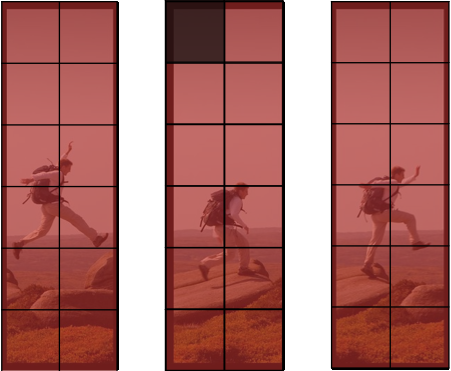
\includegraphics[scale=.50]{Images/Chapter3/openvclip_attention.png}
	\caption[]{ وصله‌های درنظر گرفته شده برای هر وصله از قاب در سازوکار تغییر یافته‌ی توجه}
	\label{fig.31}
\end{figure}

\subsection{منظم‌سازی وزن‌های میان‌یابی}
همانطور که ذکر شد، برای جلوگیری از فراموشی دانش پیش‌آموزش و در عین حال سازگار کردن مدل با داده‌های جدید، منظم‌سازی وزن‌های میان‌یابی معرفی شده است. در این روش، وزن‌های مدل به‌صورت ترکیبی از پارامتر‌های اولیه (پیش‌آموزش) و پارامتر‌های به‌روزرسانی‌شده در وظیفه جدید، تنظیم می‌شوند. این میان‌یابی به مدل کمک می‌کند تا در حین یادگیری، تعادلی میان دانش قدیمی و اطلاعات تازه برقرار کرده و از بیش‌برازش
 \LTRfootnote{Overfitting}
  جلوگیری کند. روش به‌کار رفته، تعمیم ایده‌ی گابریل و همکاران
  \cite{patchingmodels}،
 که مطابق با \eqref{eq:patching_model_base} است، می‌باشد.
\begin{equation}\label{eq:patching_model_base}
\theta = \lambda \theta_A + (1 - \lambda) \theta_B
\end{equation}

در این رابطه، $\theta$ از ترکیب خطی وزن‌های مدل پایه $\theta_A$ و مدل به‌روزرسانی‌شده $\theta_B$ با ضریب $\lambda$ تشکیل می‌شود تا صحت مدل در وظایف جدید افزایش یابد، بدون آنکه عملکرد آن در سایر وظایف که از پیش بهینه بوده‌اند، کاهش پیدا کند. با توجه به این که $\lambda$ یک ابرپارامتر \LTRfootnote{Hyper parameter} است، مقدار انتخابی آن، می‌تواند باعث بیش‌برازش یا زیربرازش روی داده‌های قبلی و جدید شود. پس به‌جای بهینه‌سازی مدل برای یک مقدار ثابت از $\lambda$، راه حلی باید ارائه شود که عملکرد مدل ترکیبی را در برابر بازه‌ای از مقادیر $\lambda$ بهینه کند. بنابراین، مطابق با \eqref{eq:patching_model_new}، وزن‌های جدید را در آموزش به سمتی می‌برد که هم زیان مدل جدید و هم زیان مدل ترکیبی با ضریب $\alpha$ روی داده‌های جدید حداقل شود. در این حالت، ترکیب‌های مختلف مدل قبلی و جدید در مراحل مختلف آموزش در نظر گرفته می‌شود که در واقع، عملکرد بهتری در تحلیل داده‌های نادیده خواهد داشت. در انتها مطابق با \eqref{eq:patching_model_base}، مدل جدید و قدیم ترکیب خواهند شد. با این تفاوت که وزن‌های مدل جدید، در طول آموزش با در نظر گرفتن عدم فراموشی مدل قبلی، یاد گرفته شده‌اند.
\begin{equation}\label{eq:patching_model_new}
	\arg \min_{\theta_B} \mathcal{L} =
	L(\theta_B; D_B) + \beta L\big(\alpha \theta_A + (1 - \alpha)\theta_B; D_B\big)
\end{equation}
پارامتر \( \alpha \) از یک توزیع یکنواخت در بازه \( (0, \lambda) \) نمونه‌برداری می‌شود و ضریب \( \beta \) به‌عنوان یک پارامتر تنظیم‌کننده برای کنترل میزان تاثیر عبارت میان‌یابی تعریف شده است. همچنین مقدار \( \beta \) به‌صورت \( \beta = C \frac{1}{1 - \alpha} \) محاسبه می‌شود که در آن \( C \) یک مقدار ثابت برای کنترل بزرگی \(\beta\) است. 

\subsection{میانگین‌گیری تصادفی وزن‌ها}
هم‌چنین به‌منظور تثبیت بیشتر مدل و بهبود قابلیت تعمیم آن، روش میانگین‌گیری تصادفی وزن‌ها\LTRfootnote{Stochastic Weight Averaging (SWA)} به کار گرفته شده است. در این مرحله، پارامتر‌های مدل جدید در طول چند مرحله از آموزش، ذخیره شده و میانگین آن‌ها به عنوان پارامتر نهایی انتخاب می‌شود. این رویکرد باعث کاهش نوسانات وزن‌ها و دستیابی به عملکرد پایدارتر در داده‌های آزمایشی می‌گردد. در نهایت، فرمول نهایی مدل مطابق با \eqref{eq:patching_model_final} خواهد بود.

\begin{equation}\label{eq:patching_model_final}
	\sum_{i}^{N} \frac{\lambda \theta_{A} + (1 - \lambda) \theta_{i}}{N}
	= \lambda \theta_{A} + (1 - \lambda)
	\left( \frac{1}{N} \sum_{i}^{N} \theta_{i} \right)
\end{equation}
بنابراین، مدل نهایی، تنظیم دقیق مدل \lr{CLIP} با تغییر سازوکار توجه بوده و برای جلوگیری از فراموشی مدل قبلی و حفظ قابلیت یادگیری بدون نمونه، دو تکنیک مناسب بکار گرفته شده است. 
\section{مدل \lr{L2P}}
روش ارائه‌شده در این مقاله، با هدف بهبود یادگیری پیوسته، از سازوکاری مبتنی بر «استخر پرامپت‌» استفاده می‌کند. در این رویکرد، به‌جای تغییر پارامتر‌های اصلی مدل، مجموعه‌ای از پرامپت‌های قابل‌آموزش طراحی می‌شود که مدل با استفاده از آن‌ها قادر به استخراج اطلاعات مهم از داده‌های ورودی است. در هر مرحله یادگیری، پرامپت‌های مناسب بر اساس شباهت با داده‌های جدید انتخاب می‌شوند و این امر باعث می‌شود مدل بتواند دانش جدید را یاد بگیرد، بدون آنکه دانش قبلی را فراموش کند. این روش با بهره‌گیری از معماری ترنسفورمر، توانسته است تعادل موثری میان حفظ دانش گذشته و یادگیری وظایف جدید برقرار کند. همانطور که در \cref{fig.32} قابل مشاهده است، این مدل دارای دو بخش انتخاب پرامپت‌ها و یادگیری و به‌روزرسانی پرامپت‌ها است که هر یک در ادامه توضیح داده‌ می‌شود.
‌\begin{figure}
	\centering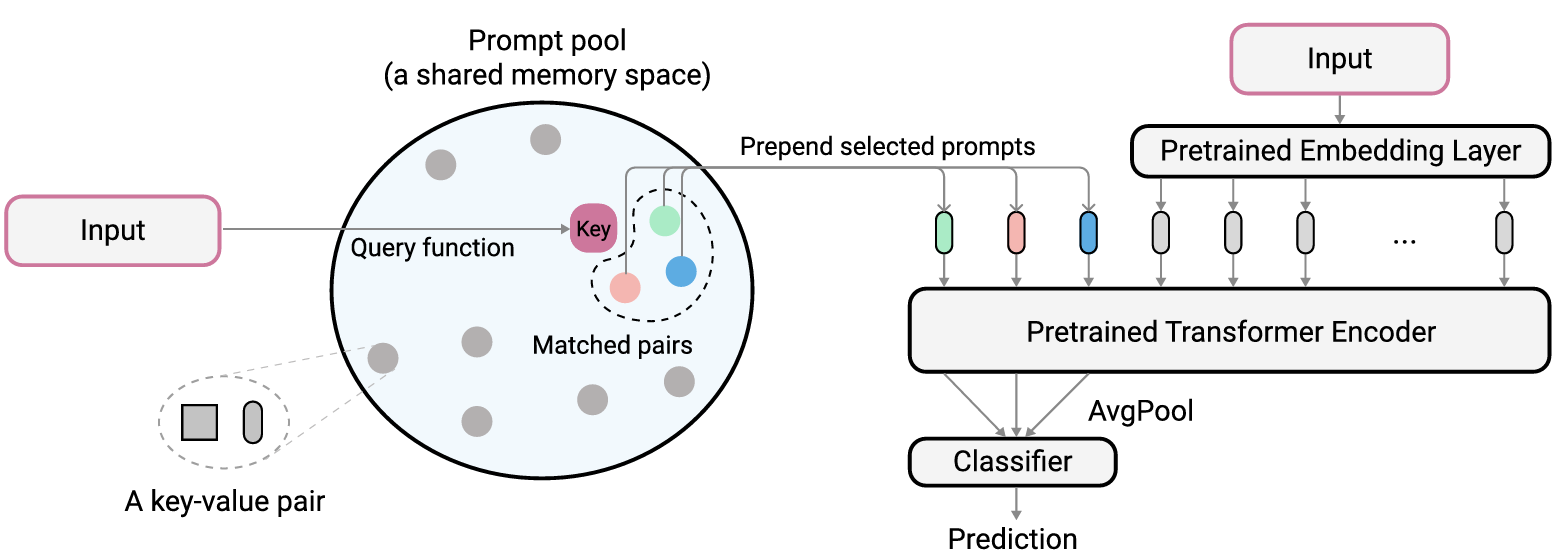
\includegraphics[scale=.38]{Images/Chapter3/l2p.png}
	\caption[]{ طرح کلی مدل \lr{L2P} \cite{l2p}}
	\label{fig.32}
\end{figure}

\subsection{انتخاب پرامپت}
در بخش انتخاب پرامپت\LTRfootnote{Prompt selection}، از استخر پرامپت تعدادی پرامپت متناسب با ورودی تصویری انتخاب می‌شود. استخر پرامپت شامل تعدادی پرامپت به تعداد $M$ بوده که به صورت \(\mathbf{P} = \{ P_{1}, P_{2}, \cdots, P_{M} \}\) نمایش داده‌ می‌شوند. هر \( P_j \in \mathbb{R}^{L_p \times D} \) یک پرامپت منفرد با طول نشانه‌ی \( L_p \) و اندازه تعبیه‌ی $D$ \LTRfootnote{Embedding size} مشابه تعبیه‌ی ورودی است. هم‌چنین هر پرامپت، دارای یک کلید است و فرآیند انتخاب بر اساس شباهت این کلیدها با بردار ویژگی مرتبط با کلاس ورودی انجام می‌گیرد. بردار ویژگی موردنظر از طریق استخراج‌کننده‌ی ویژگی، به‌دست می‌آید و سپس با کلیدهای موجود در استخر مقایسه می‌شود. در نهایت، تعدادی از پرامپت‌های کلیدهایی که بیشترین شباهت را با بردار ویژگی دارند انتخاب می‌شوند (مطابق با \cref{fig.32}). مجموعه‌ای از کلیدها به‌صورت 
\(\mathbf{K} = \{k_{j}\}_{i=1}^{M}\) 
نمایش داده می‌شود که هر \(k_i \in \mathbb{R}^{D_k}\) است. استخراج‌کننده‌ی ویژگی به صورت  \( q : \mathbb{R}^{H \times W \times C} \to \mathbb{R}^{D_k} \) معرفی می‌شود که بردار ویژگی \(x\) را به همان بعد کلیدها نگاشت می‌کند. در واقع از مدل ازپیش‌آموزش‌دیده به‌عنوان استخراج‌کننده ویژگی منجمد \LTRfootnote{Frozen} استفاده می‌شود:
\( q(x) = f(x)[0,:] \)
(که در آن از بردار ویژگی متناظر با کلاس استفاده می‌شود). 
تابع \(\gamma : \mathbb{R}^{D_k} \times \mathbb{R}^{D_k} \to \mathbb{R}\) به‌عنوان معیاری برای سنجش میزان تطابق بین بردار ویژگی ورودی و کلید پرامپت تعریف می‌شود (مانند فاصله کسینوسی). برای یک ورودی \(x\)، از تابع \(q(x)\) استفاده می‌کنیم تا بهترین \(N\) کلید انتخاب شوند. در نهایت، انتخاب کلید طبق \eqref{eq:prompt_selection} صورت می‌گیرد.
\begin{equation}\label{eq:prompt_selection}
	\mathbf{K}_x = 
	\underset{\{s_i\}_{i=1}^{N} \subseteq [1, M]}{\arg\min} 
	\sum_{i=1}^{N} \gamma \big( q(x), \mathbf{k}_{s_i} \big),
\end{equation}
\(\{s_i\}_{i=1}^{N}\) به‌عنوان یک زیرمجموعه از \(N\) کلید از بازه \([1, M]\) در نظر گرفته می‌شود
و \( \mathbf{K}_x \) نشان‌دهنده یک زیرمجموعه از بهترین \( N \) کلید انتخاب‌شده از \( \mathbf{K} \) به‌طور خاص برای نمونه \( x \) است.

علاوه بر این، به روش انتخاب پرامپت، قابلیت اضافه‌ای نیز اضافه شده است به این صورت که برای پرامپت‌های قبلا به‌روزرسانی شده، جریمه در نظر گرفته است تا متناسب با تعداد تکرارشان در وظایف قبلی، جریمه‌ی بیشتری برای انتخاب بگیرند. در این حالت، پرامپت‌های با تکرار کم نیز شانس انتخاب شدن پیدا می‌کنند و پرامپت‌ها با تکرار بیشتر، کمتر تغییر می‌کنند و تداخل کمتر می‌شود.
\subsection{یادگیری پرامپت}
در بخش یادگیری پرامپت، پرامپت‌های انتخاب‌شده به‌همراه داده‌ی ورودی به مدل تغذیه شده و پس از عبور از لایه‌های ترنسفورمر، بخش خروجی مربوط به پرامپت‌ها، استخراج شده و با میانگین‌گیری، به دسته‌بند \LTRfootnote{Classifier} منتقل می‌شود. سپس با انجام عملیات پس‌انتشار \LTRfootnote{Backpropagation}، وزن‌های پرامپت‌ها و کلیدهای متناظر آن‌ها به‌روزرسانی می‌شوند. این فرآیند باعث می‌شود مدل ضمن یادگیری وظایف جدید، قابلیت تعمیم خود را افزایش داده و دانش قبلی را حفظ کند (مطابق با \cref{fig.32}). تابع زیان در این مدل مطابق با \eqref{eq:l2p_loss}، به صورت ترکیبی معرفی می‌شود به این صورت که بخش اول شامل زیان بین برچسب تصویر و پیش‌بینی دسته‌بند از ورودی دارای پرامپت و بخش دوم شامل تفاوت بین کلیدهای انتخاب شده و ویژگی استخراجی از ورودی می‌باشد. به عبارتی تلاش بر این است که علاوه بر تقویت پرامپت‌ها، کلیدهای مرتبط نیز، به ویژگی ورودی متناظرشان نزدیک‌‌‌تر شوند. 
\begin{equation}\label{eq:l2p_loss}
	\min_{\mathbf{P}, \mathbf{K}, \phi} 
	\mathcal{L}\big( g_{\phi}( f_r^{\mathrm{avg}} (x_p) ), y \big) 
	+ \lambda \sum_{\mathbf{K}_x} \gamma \big( q(x), \mathbf{k}_{s_i} \big)
\end{equation}
همانطور که دیده می‌شود، بخش اول شامل تابع زیان (کراس انتروپی) بین خروجی دسته‌بند \(g_{\phi}\) و برچسب واقعی \(y\) محاسبه می‌شود. تابع \( f_r^{\mathrm{avg}} = \mathrm{AvgPool}(f_r(x_p)[0 : N L_p, :]) \)، به این معناست که بردارهای پنهان خروجی متناظر با مکان‌های \( N \cdot L_p \) پرامپت‌ها، پیش از ورود به لایه‌ی دسته‌بند، به‌صورت میانگین‌گیری شده ترکیب می‌شوند. 
در عبارت \( f_r(x_p) \)، تابع \( f_r \) نشان‌دهنده بخش باقی‌مانده از مدل ازپیش‌آموزش‌دیده است که پس از الحاق پرامپت‌ها به ورودی، عملیات پردازش ویژگی را انجام می‌دهد. 
بردار \( x_p \) نیز از اتصال پرامپت‌ها به بردار تعبیه‌شده ورودی حاصل می‌شود. در بخش دوم، پارامتر \(\lambda\) وزن اهمیت عبارت تنظیم‌کننده را مشخص می‌کند. فاصله بین بردار \(q(x)\) و کلیدهای انتخاب‌شده \(\mathbf{k}_{s_i}\) را کاهش می‌دهد. مجموعه \(\mathbf{K}_x\) نیز نشان‌دهنده کلیدهای انتخاب‌شده برای ورودی \(x\) است که طبق معادله \eqref{eq:prompt_selection} به دست می‌آیند.

در ادامه به توضیح مدل پیشنهادی و اجزای آن پرداخته می‌شود. 
\section{مرحله‌ی آموزش \lr{ProActionCLIP}}
همانطور که پیش‌تر اشاره شد، در مرحله‌ی آموزش، تمرکز بر یادگیری پرامپت‌های مناسب برای دسته‌های مختلفی است که به صورت پیوسته به مدل اضافه می‌شوند. طرح کلی مدل در مرحله‌ی آموزش در \cref{fig.33}، نشان داده شده است که الگو گرفته از مدل \lr{CLIP} می‌باشد. این مدل شامل یک کدگذار ویدیو (قابل به‌روزرسانی) و کدگذار متن منجمد (غیر قابل به‌روزرسانی) از مدل \lr{Open-VCLIP} است به این صورت که بردار ویژگی ویدیوی استخراج شده از کدگذار ویدیو و بردارهای ویژگی برچسب‌های موجود استخراج شده از کدگذار متن، طبق روش تقابلی مقایسه شده و طبق نزدیک شدن موارد متناظر و دور شدن موارد نامتناظر، وزن‌های پرامپت‌ها تغییر داده می‌شوند. دو بخش اصلی مدل به نام کدگذار ویدیو و یادگیری پرامپت در ادامه توضیح داده خواهند شد. 
‌\begin{figure}
	\centering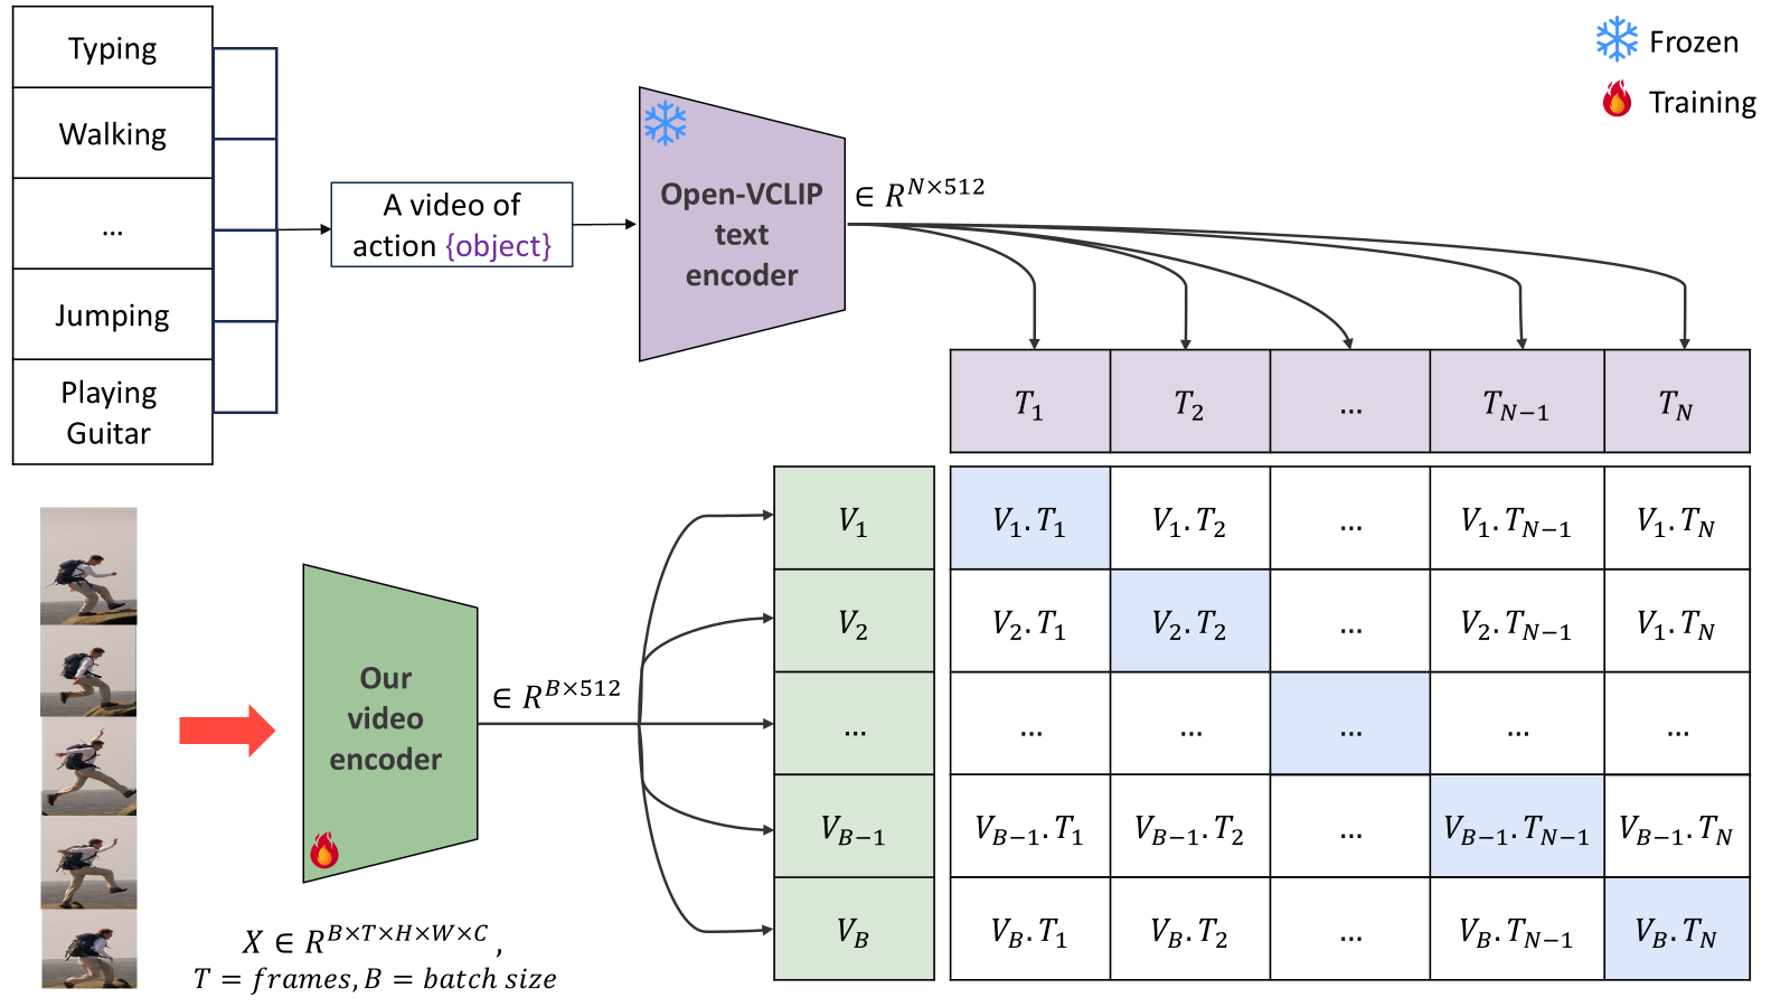
\includegraphics[scale=.50]{Images/Chapter3/train_phase.png}
	\caption[]{طرح کلی مرحله‌ی آموزش مدل \lr{ProActionCLIP}}
	\label{fig.33}
\end{figure}
\subsection{کدگذار ویدیو}
این بخش، از ترکیب \lr{L2P} و \lr{Open-VCLIP} تشکیل شده است. به طور کلی مطابق \cref{fig.34}، ویدیو به عنوان ورودی، وارد کدگذار \lr{Open-VCLIP} و لایه‌ی کانولوشنی دو‌بعدی می‌شود. ویژگی کلاس \LTRfootnote{Class feature (CLS)} از خروجی کدگذار \lr{Open-VCLIP} با 512 بعد، با کلیدهای داخل استخر پرامپت مقایسه می‌شود. به تعداد $N$ پرامپت از مشابه‌ترین کلیدها انتخاب می‌شوند. از طرف دیگر ویدیو از لایه‌ی کانولوشنی عبور کرده و پرامپت‌ها به هر قاب، به صورت جداگانه متصل می‌شوند. سپس به کدگذار ترنسفورمر معرفی شده در \lr{Open-VCLIP}، وارد شده و به ازای هر قاب، یک ویژگی کلاس بدست می‌آید که میانگین آن‌ها محاسبه و به عنوان خروجی نهایی این بخش، ارائه می‌گردد. در مدل پیشنهادی، صرفا پرامپت‌ها و کلیدهای متناظر آن‌ها، قابل یادگیری هستند و بقیه‌ی اجزا به صورت منجمد استفاده می‌شوند. در این بخش از تحقیق، آزمایش‌های مختلفی اجرا شد که بر اساس نوع انتخاب پرامپت و شرایط استخر پرامپت می‌توان به دسته‌‌های زیر تقسیم نمود:
\begin{itemize}
\item \textbf{مقداردهی اولیه‌ی کلید پرامپت:}
از آن جایی که ابتدای آموزش، مقادیر اولیه به صورت تصادفی هستند، در این آزمایش، مقادیر کلیدها، معادل ویژگی‌های برچسب دسته‌های استخراج شده از کدگذار متن قرار داده شد. در این صورت، مقایسه‌ی ویژگی ویدیو و کلیدها به صورت بهینه‌تر و دقیق‌تری صورت می‌گیرد. 
\item \textbf{وزن‌دهی به کلید پرامپت‌های از قبل انتخاب شده:}
مطابق با روش اضافه‌ای که برای انتخاب پرامپت در \lr{L2P} مطرح شد، تعداد تکرار پرامپت‌ها در هر وظیفه محاسبه می‌شود. در وظیفه‌ی بعدی، هرچه تکرار پرامپت بیشتر بوده باشد، تاثیرش در انتخاب کمتر می‌شود. 
\item \textbf{منجمد کردن پرامپت‌های قبلی:}
یکی از راه‌های استفاده از وزن‌های قبلی، این است که به صورت منجمد استفاده شوند و به‌روزرسانی نشوند. این روش کمک می‌کند اطلاعات اختصاصی هر وظیفه از بین نرود و اگر داده‌ی جدید اشتراکی با قبلی‌ها داشته باشد، پرامپت آن‌ها را انتخاب خواهد کرد.
\item \textbf{پویا بودن تعداد پرامپت‌های استخر پرامپت:}
در فرض اولیه، در استخر پرامپت تعدادی ثابت پرامپت وجود داشت اما برای بهینه‌بودن مدل برای دسته‌های بیشتر و موجود بودن پرامپت کافی در هر وظیفه، در این قسمت پرامپت‌ها در ابتدای هر وظیفه افزایش میابد. 

ترکیب برخی از این روش‌ها نیز آزمایش شده است مانند استفاده از استخر پویا و مقداردهی اولیه کلیدها.  
\end{itemize}
\begin{figure}
	\centering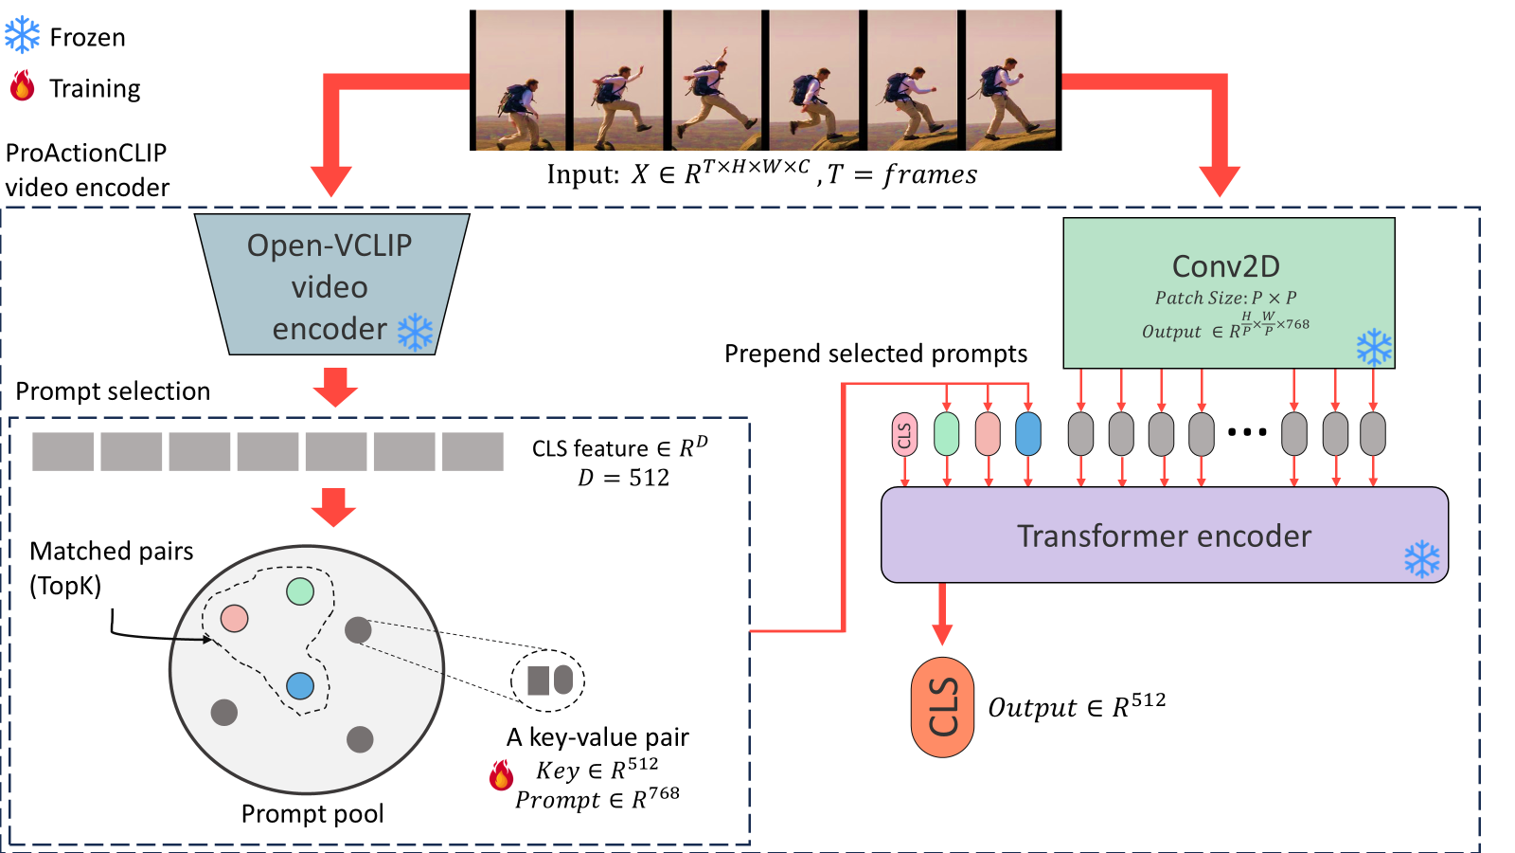
\includegraphics[scale=.65]{Images/Chapter3/video_encoder.png}
	\caption[]{سازوکار بخش کدگذار ویدیو مدل \lr{ProActionCLIP}}
	\label{fig.34}
\end{figure}
\subsection{یادگیری پرامپت}
وقتی ویدیو از کدگذار ویدیوی پیشنهادی عبور کرد، وارد مرحله‌ی نهایی برای به‌روزرسانی وزن‌های پرامپت‌ها و کلید‌های متناظرشان می‌شود. مطابق با \cref{fig.33}، ویژگی برچسب‌ها از طریق کدگذار متن مدل \lr{Open-VCLIP} بدست می‌آید. تابع زیان همانند روش \lr{L2P}، شامل دو بخش است. اولین بخش شامل زیان بین ویژگی استخراجی از ویدیو و ویژگی برچسب متناظر آن و بخش بعدی مختص زیان بین ویدیو و کلیدهای انتخاب شده برای آن می‌باشد. در این صورت پرامپت‌ها در بخش اول و کلیدها در بخش دوم تابع زیان مورد تمرکز قرار می‌گیرند. تابع زیان مدل پیشنهادی با \lr{L2P} تفاوت‌هایی دارد که در ادامه بررسی می‌کنیم. روش مدل پیشنهادی برگرفته از مدل \lr{CLIP}، برخلاف \lr{L2P} که با دسته‌بند است، به صورت تقابلی می‌باشد. مطابق \eqref{eq:our_loss}، پرامپت‌های انتخابی، به ورودی عبور کرده از لایه‌ی کانولوشنی، ملحق شده و $x_{p,t}$ را تشکیل می‌دهند. $t$ نشان‌دهنده‌ی هر قاب است. سپس از لایه‌ی ترنسفورمر معرفی شده، عبور کرده و به صورت $z(x_{p,t})$ نمایش داده می‌شود. خروجی ترنسفورمر، در بردارهای ویژگی برچسب‌ها که از کدگذار متن بدست آمده ($W$)، ضرب می‌شود. از $\tau$ نیز به عنوان ضریب مقیاس‌دهی در این ضرب استفاده می‌شود. در این حالت شباهت ویژگی بدست آمده از قاب $t$ از ویدیو، با برچسب‌ها سنجیده می‌شود. سپس میانگین شباهت‌ها برای قاب‌های ویدیو ($T$) محاسبه می‌شود. تابع زیان کراس انتروپی بین خروجی و برچسب‌ متناظر اجرا می‌شود. بخش دوم، مانند روش \lr{L2P}، بر نزدیک کردن کلیدهای انتخاب شده، به ویژگی کلاس ویدیوی نمونه، سعی دارد که در بخش قبل به تفصیل شرح داده شد.
\begin{equation}\label{eq:our_loss}
	\mathcal{L} = \mathrm{CE} \left( 
	\frac{1}{T} \sum_{t=1}^{T} 
	\left[ 
	\mathbf{\tau \cdot z(x_{p,t})} \mathbf{W}^{\mathrm{T}} 
	\right], 
	y 
	\right) 
	+ \lambda \sum_{\mathbf{K}_x} \gamma \big( q(x), \mathbf{k}_{s_i} \big)
\end{equation}
% \exp(\mathrm{logitscale}) \cdot 

\section{مرحله‌ی آزمون \lr{ProActionCLIP}}
برای آزمون مدل، مطابق \cref{fig.35}، ویدیو وارد کدگذار ویدیو می‌شود و به تعداد $N$ نزدیکترین کلید به ویژگی ویدیو، را انتخاب کرده و به هر یک از قاب‌های ویدیو ملحق کرده و از ترنسفورمر عبور می‌دهد. خروجی نهایی این بخش را با ویژگی استخراج شده‌ی برچسب‌ها از کدگذار متن، مقایسه کرده و برچسب با بیشترین شباهت انتخاب می‌شود.
‌\begin{figure}
	\centering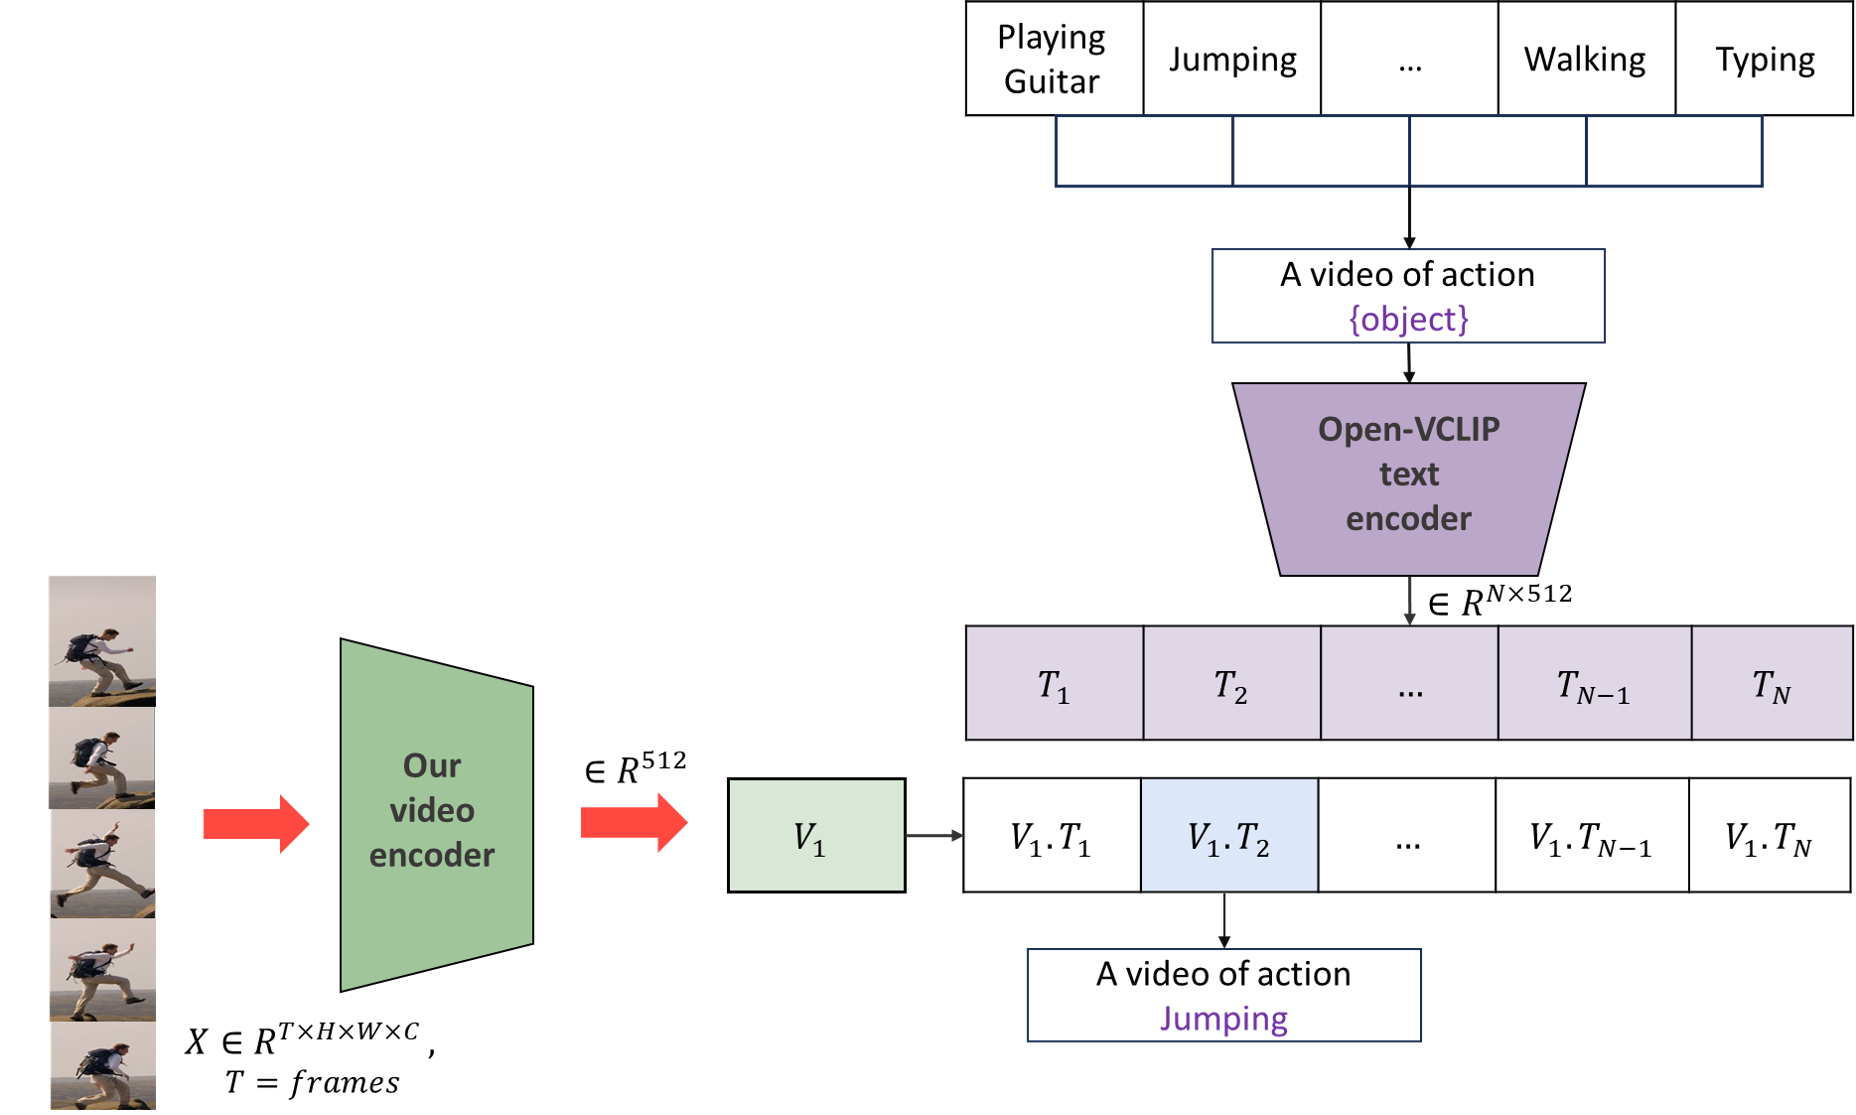
\includegraphics[scale=.48]{Images/Chapter3/test_phase.png}
	\caption[]{طرح کلی مرحله‌ی آزمون مدل \lr{ProActionCLIP}}
	\label{fig.35}
\end{figure}
\section{جمع‌بندی}
در این فصل مدل نهایی پیشنهادی این پژوهش با نام \lr{ProActionCLIP} معرفی شد که ترکیبی از دو مدل \lr{L2P} و \lr{Open-VCLIP} بوده که با تلفیق قابلیت یادگیری پرامپت در \lr{L2P} و توانایی استخراج ویژگی‌های ویدیویی در \lr{Open-VCLIP} طراحی شده است. در این فصل، ساختار کلی مدل پیشنهادی و اجزای اصلی آن شامل کدگذار ویدیو، کدگذار متن منجمد و سازوکار یادگیری پرامپت تشریح شد. تکنیک‌های مختلف استفاده شده در طراحی استخر پرامپت‌ها و روش انتخاب پرامپت‌های مناسب برای هر ورودی، نیز شرح داده شد. همچنین نحوه تعامل این اجزا با یکدیگر برای یادگیری پیوسته و به‌روزرسانی وزن‌های پرامپت‌ها از طریق الگوریتم پس‌انتشار توضیح داده شد. در نهایت، فرآیند آموزش مدل و محاسبه تابع زیان که شامل عبارت منظم‌سازی (برای نزدیک کردن کلیدها و ویژگی ویدیو) و معیار تقابلی است، مورد بررسی قرار گرفت.


